\documentclass[aspectratio=169]{beamer}
\usepackage[utf8]{inputenc}
\usepackage{transparent}
\usepackage{hyperref}
\usepackage{pgf}
\usepackage{dsfont}
\usepackage{algorithm}
\usepackage{algorithmic}

% here comes my custom theme for university of Bamberg

\logo{\pgfputat{\pgfxy(-1.25,4.25)}{\pgfbox[center,base]{\transparent{0.7} 
\includegraphics[width=.15\textwidth]{uni_bamberg.png}}}}


\newcommand{\nologo}{\setbeamertemplate{logo}{}} % command to set the logo to nothing
\newcommand{\biglogo}{\setbeamertemplate{logo}{\pgfputat{\pgfxy(-2,4)}{\pgfbox[center,base]{ 
\includegraphics[width=.24\textwidth]{uni_bamberg.png}}}}} 

% theming and colors and stuff
\usetheme[progressbar=frametitle, block = fill]{metropolis}
\definecolor{uniblau}{RGB}{4, 66, 119} %#044277
\definecolor{niceorange}{RGB}{255, 128, 0} %#ff8000
\definecolor{nicegray}{RGB}{221, 239, 244} %#ddeff4
\setbeamercolor{palette primary}{bg=uniblau, fg=white}
\setbeamercolor{normal text}{fg=uniblau, bg=white}
\setbeamercolor{itemize item}{fg=niceorange}
\setbeamercolor{itemize subitem}{fg=niceorange}
\setbeamercolor{itemize subsubitem}{fg=niceorange}
\setbeamercolor{enumerate item}{fg=niceorange}
\setbeamercolor{enumerate subitem}{fg=niceorange}
\setbeamercolor{enumerate subsubitem}{fg=niceorange}
\setbeamercolor{block body}{bg=nicegray}
\setbeamercolor{block title}{bg=niceorange,fg=white}
\renewcommand\UrlFont{\color{niceorange}\rmfamily}

% own commands for highlighting
\newcommand{\pop}[1]{{\color{niceorange}\textbf{#1}}}

\def\ps@titlepage{\setbeamertemplate{footline}{}}
\makeatletter
\setbeamertemplate{frame footer}{\tiny{xAI-Proj-M - Data Engineering - J.Amling }}

% custom python style

%title page
\title{Data Engineering  -- Background Removal}
\subtitle{Explainable Machine Learning - Deep Learning Life Cycle}
\author{Jonas Amling \and Baptiste Patrice Francis Bony \and Benedikt Markus Marsiske}
\institute{University of Bamberg}
\date{\today} 

\begin{document}
% titleframe
{\biglogo
	\setbeamertemplate{footline}{} 
	\begin{frame}{}
		\titlepage
	\end{frame}
}

\begin{frame}{Table of contents}
	\tableofcontents
\end{frame}


{\nologo
\section{Research Question}
	\begin{frame}{Research Question and Introduction}
	Our main Data Engineering Problems:
	\begin{itemize}
		\item Combining different datasets
		\item Different hand positions in different datasets
		\item Hands in different contexts in each dataset
		\pause
		\item	$\implies$ reducing complexity of datasets is key
	\end{itemize}
	\pause
	Research Question: \pop{Does removing the background during the image preprocessing phase benefit the image classification task at hand?} 
	\end{frame}

\section{Data Engeneering Process}
	\begin{frame}{Problem Description}
	Several Problems have to be solved in the preprocessing stage
	\begin{itemize}
		\item data selection:
		\begin{itemize}
			\item cgi, 
			\item real-hands or 
			\item self generated data
		\end{itemize}
		\pause
		\item standardize/normalize hand positions from different datasets
		\pause
		\item all images have to be processed by only ONE preprocessor
	\end{itemize}
	\end{frame}
	
	\begin{frame}{Existing libraries}
	Searching the WWW we found some interesting libraries:
	\begin{itemize}
		\item YOLO-Hand-Detection: find hand position in an image \footnote{https://github.com/cansik/yolo-hand-detection}
		\begin{itemize}
			\item[+] works on real life images, open source
			\item[-] not included in Python Package Index
		\end{itemize}
		\pause
		\item rembg: model that automatically removes image background \footnote{https://pypi.org/project/rembg/}
		\begin{itemize}
			\item[+] comes as library in Python Package Index 
			\item[-] not works in all cases, has some strange edge cases
		\end{itemize}
		\pause
		\item MediaPipe Hands: generates a 3d hand model from a 2d image \footnote{https://google.github.io/mediapipe/solutions/hands.html}
		\begin{itemize}
			\item[+] works quite well and comes as library in Python Package Index 
			\item[-] developed by google
		\end{itemize}
	\end{itemize}
	% YOLO library
	% rembg library
	% mediapipe
	\end{frame}
	
	\begin{frame}{Our Preprocessor}
	Parameters for Image Processing:
	\begin{itemize}
		\item desired dimensions  of preprocessed image
		\item crop image, based on the hand position within the image
		\item remove background
	\end{itemize}
	Preprocessing steps:
	\begin{enumerate}
	\item read image using cv2
	\item crop image based on bounding-box found with MediaPipe
	\item remove left over background using rembg library
	\item resize image and add padding if necessary
	\end{enumerate}
	\end{frame}
	
	
	\begin{frame}{Preprocessing Examples -- a good one}
% start the columns environment and set the
% positioning of the content inside the columns at
% the top with the T specifier
\begin{columns}[c]
% create the column with the first image, that occupies
% half of the slide
    \begin{column}{.33\textwidth}
    \begin{figure}
        \centering
        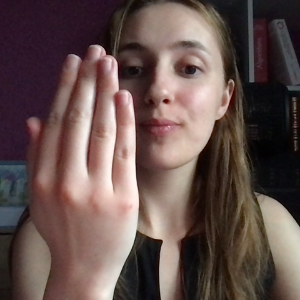
\includegraphics[width=0.9\textwidth]{img/test/nasmi_203.png}
        \caption{original}
    \end{figure}      
    \end{column}
% create the column with the second image, that also
% occupies half of the slide
    \begin{column}{.33\textwidth}
    \begin{figure}
        \centering
        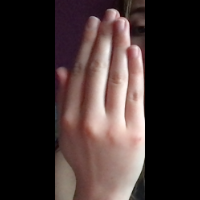
\includegraphics[width=0.9\textwidth]{img/cropped/nasmi_203.png}
        \caption{cropped}
    \end{figure}
    \end{column}
    
    \begin{column}{.33\textwidth}
    \begin{figure}
        \centering
        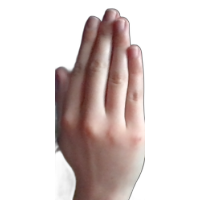
\includegraphics[width=0.9\textwidth]{img/rembg/nasmi_203.png}
        \caption{background removal}
    \end{figure}
    \end{column}
\end{columns}
\end{frame}

\begin{frame}{Preprocessing Examples -- a not so good one}
% start the columns environment and set the
% positioning of the content inside the columns at
% the top with the T specifier
\begin{columns}[c]
% create the column with the first image, that occupies
% half of the slide
    \begin{column}{.33\textwidth}
    \begin{figure}
        \centering
        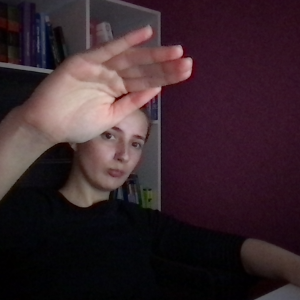
\includegraphics[width=0.9\textwidth]{img/test/nasmi_304.png}
        \caption{original}
    \end{figure}      
    \end{column}
% create the column with the second image, that also
% occupies half of the slide
    \begin{column}{.33\textwidth}
    \begin{figure}
        \centering
        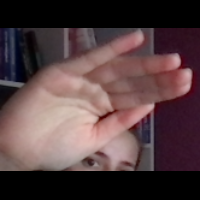
\includegraphics[width=0.9\textwidth]{img/cropped/nasmi_304.png}
        \caption{cropped}
    \end{figure}
    \end{column}
    
    \begin{column}{.33\textwidth}
    \begin{figure}
        \centering
        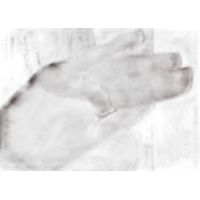
\includegraphics[width=0.9\textwidth]{img/rembg/nasmi_304.png}
        \caption{background removal}
    \end{figure}
    \end{column}
\end{columns}
\end{frame}

\section{Future Considerations}
	\begin{frame}{Discussion}
	Things we will have to consider for the future project
	\begin{itemize}
		\item is there a better library than rembg
		\item how much data do we want use
		\item do we want to train on color or greyscale images
		\item what is the exact setting in which we want to use our deep learning model
	\end{itemize}
	\end{frame}
}



% finally our last stuff
\appendix
{\nologo
	\begin{frame}[standout]
		Thank you!
	\end{frame}

    
	\begin{frame}[allowframebreaks]{References}
	
	\bibliographystyle{ieeetr}
  	\bibliography{references}
  	

	\end{frame}
}
\end{document}